\subsection{Deployment}
\label{subs:deployment}

Die einzige Anforderung, welche das Deployment direkt betrifft, ist die 
\ref{nfa7}. Diese besagt lediglich, dass dies möglichst einfach und von außerhalb möglich
sein soll.\\
Bei nativen Applikation wäre hier ein Updater denkbar. Also ein Service,
welcher regelmäßig die Verfügbarkeit neuer Versionen auf einem Server prüft und einen Download 
dieser anbietet. Electron bietet für diesen Fall einige Möglichkeiten, diesen Prozess 
möglichst simpel zu gestalten. Beispielsweise mit dem eigenen 
\texttt{autoUpdater}-Modul \cite{electron-autoUpdater} oder Plugins wie 
\emph{electron-builder} \cite{electron-builder}. Auch sind mit beiden Möglichkeiten
automatische Updates umsetzbar.\\
Im Falle einer Applikation, die einzig mit Browsertechnologien implementiert wurde, sind 
noch simplere Strategien denkbar. Hier ist ein normales Webhosting der Applikationsdateien 
bereits eine ausreichende Deployment-Strategie. Wurde keine Offline-Verfügbarkeit durch
Service-Worker implementiert, können die statischen Files einer Browseranwendung
auch einfach auf dem Filesystem der Workstation hinterlegt und in einem Browser aufgerufen 
werden. Eventuelle Updates müssten in diesem Falle aber vor Ort oder durch einen
Fernzugriff auf den Rechner eingespielt werden. Im Fall des Webhostings genügt das Überspielen
der neuen Files auf einen Webserver.\\

\begin{figure}
    \centering
    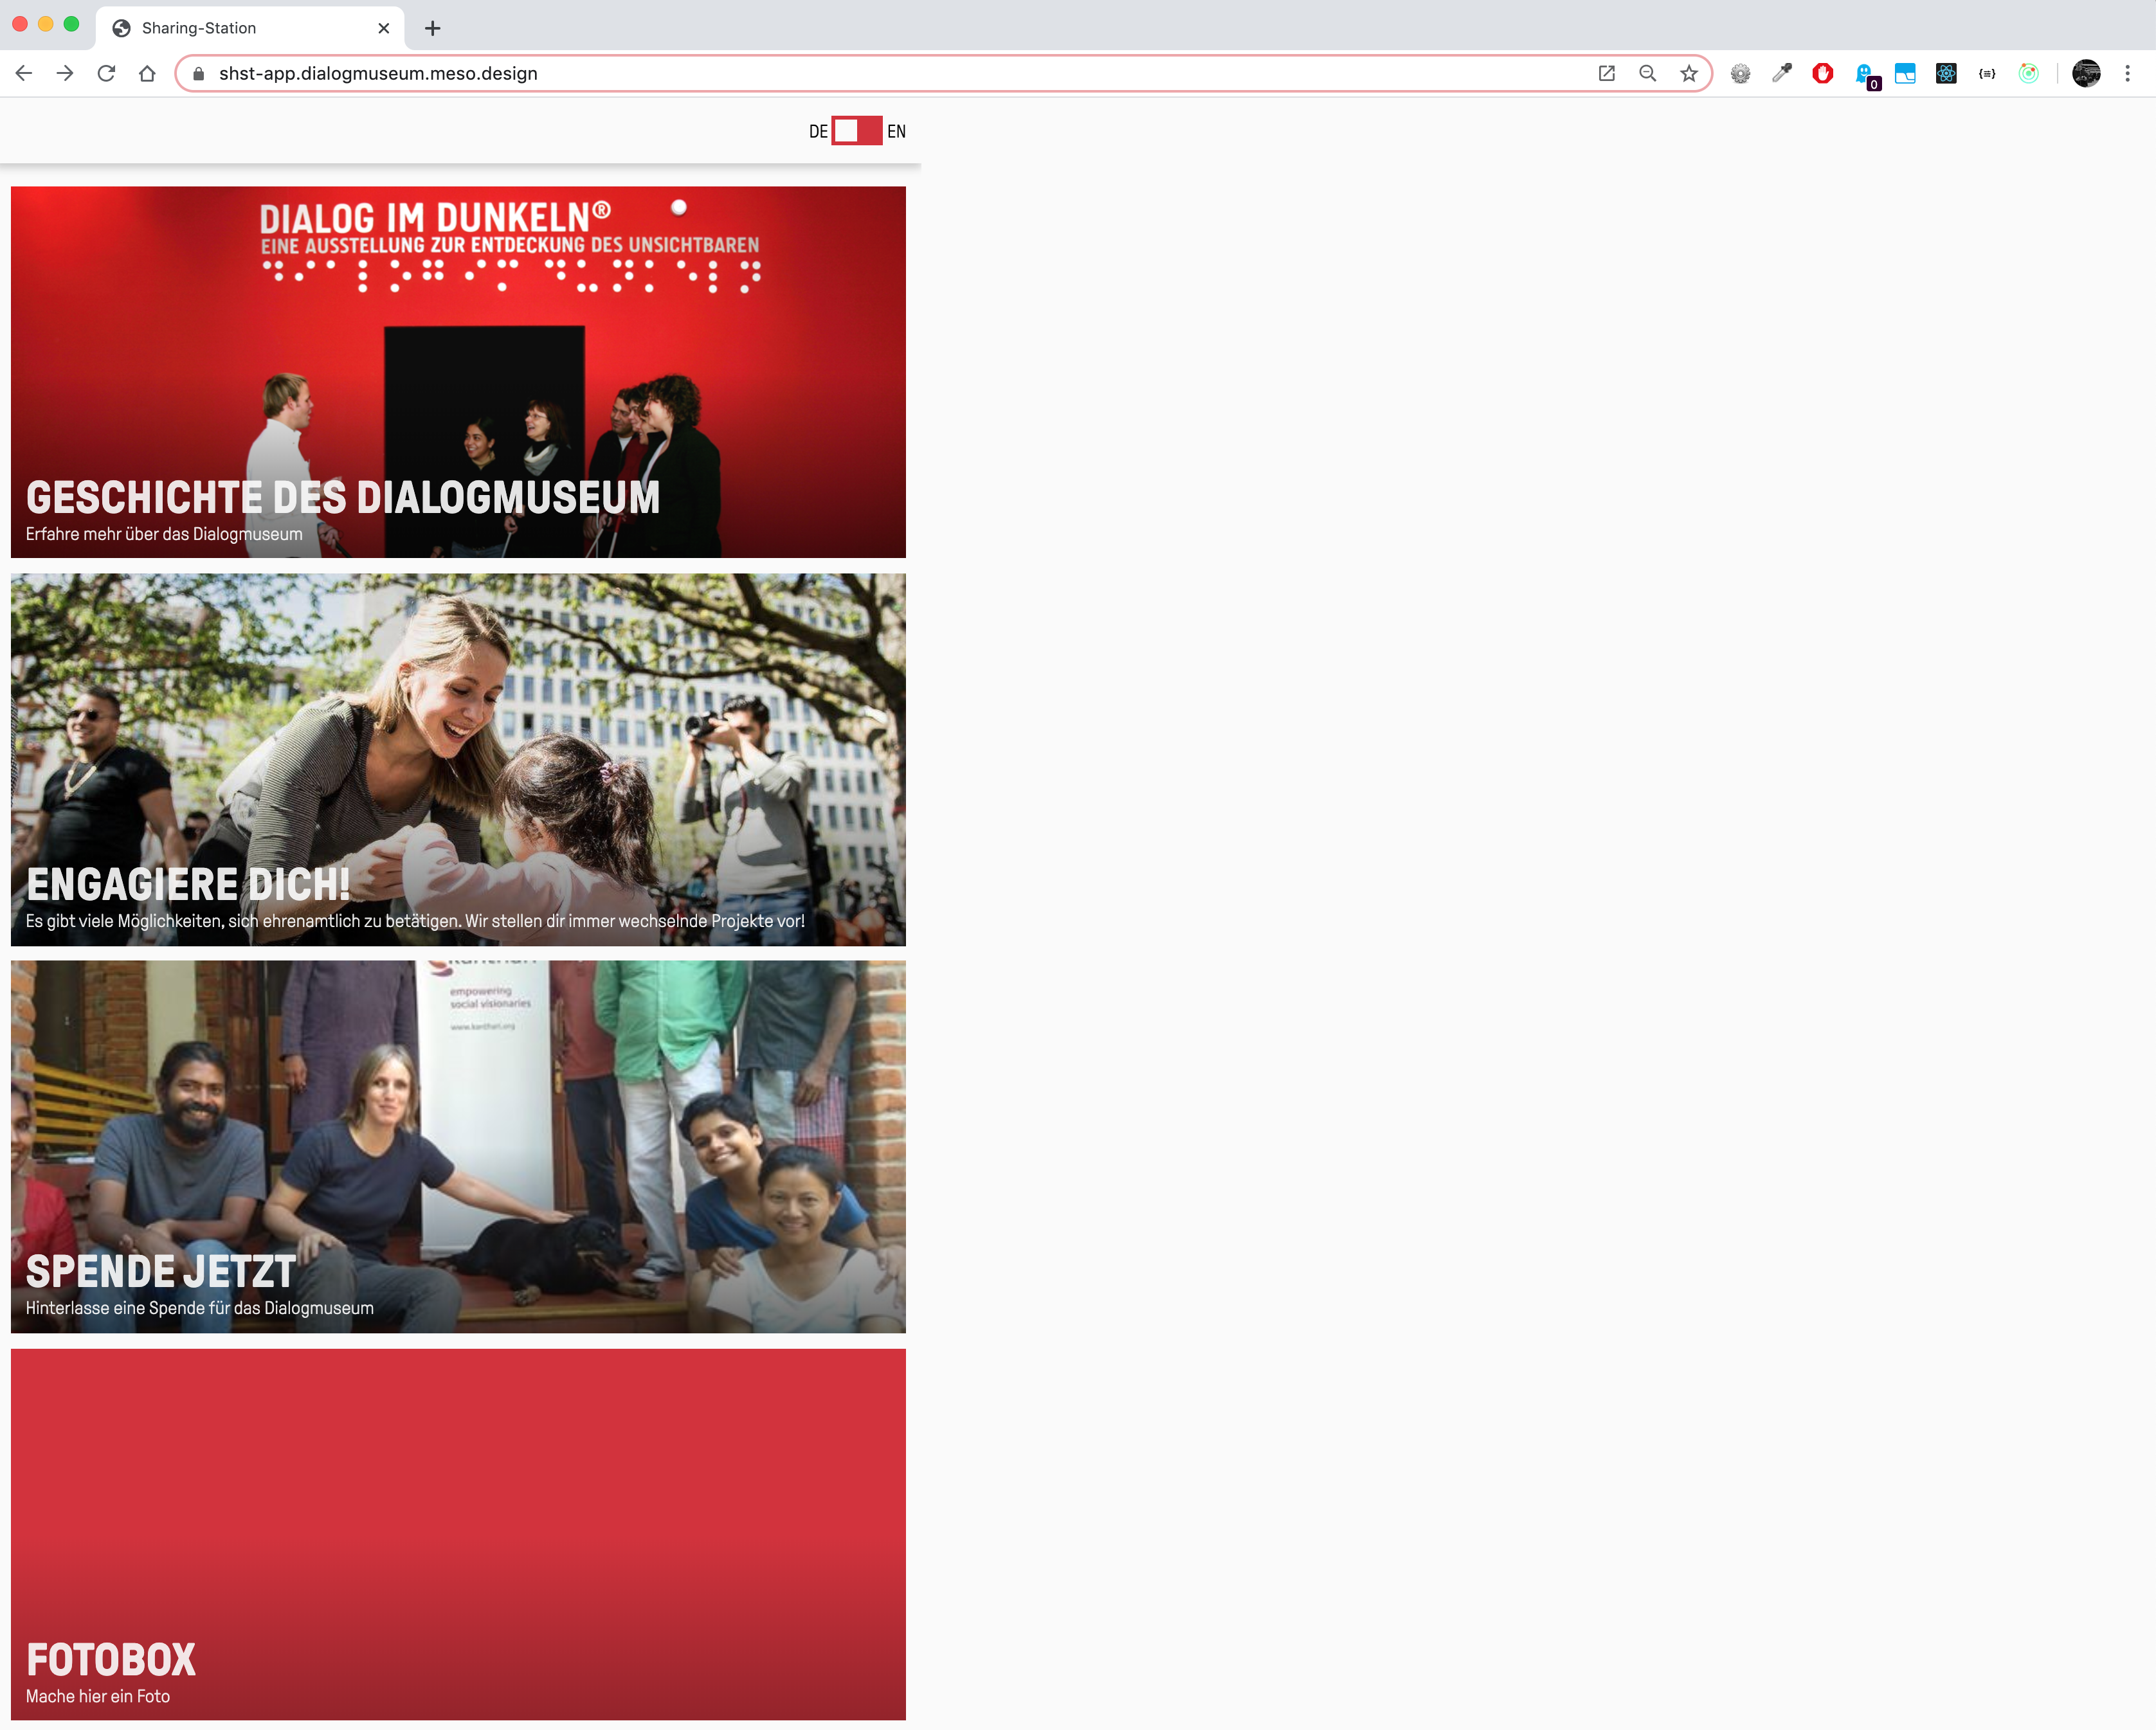
\includegraphics[width=1\textwidth]{figures/images/browser-preview.png}
    \caption{Vorschau der \shst{} Clientanwendung im Browser}
    \label{fig:browser-preview}
\end{figure}

Für die \shst{} wurde auf dem Server neben dem CMS auch ein Webserver installiert, welcher die 
Applikationsdateien ausliefert (\autoref{fig:ss-deployment-diagram}). Zusätzlich wurde über den 
firmeninternen GitLab-Server \cite{gitlab} eine Build- und Deployment-Pipeline eingerichtet, welche die 
Applikationsdateien automatisch generiert und vom Master-Branch des Repositorys auf den Webserver überträgt. 
Für ein Update der Clientanwendung auf der Workstation in der Ausstellung ist also nichts weiter 
nötig, als die Änderungen auf den Master-Branch des Repositorys zu übertragen und die Applikation vor
Ort neu zu laden.\\
Das Webhosting der Applikation bietet außerdem den Vorteil, dass diese jeder Zeit in einem Browser 
über das Internet aufgerufen werden kann. Beim Anlegen von Daten im CMS kann dies so als
Vorschau genutzt werden (\autoref{fig:browser-preview}). 